\chapter{Introduzione}

%%%%%% OBIETTIVI %%%%%%%%
\section{Obiettivi del progetto}
Il seguente progetto di tesi si pone l’obiettivo di trovare delle relazioni tra diversi indici bibliometrici che vengono utilizzati 
per valutare la produzione accademica. 
Una visione complessiva dei dati può essere utile per valutare gli andamenti e migliorare la produttività accademica. 
L’applicazione sviluppata permette, tramite interfaccia grafica, di gestire e visualizzare autori, paper, università e conferenze, 
interfacciandosi con un database per l’inserimento e l’interrogazione dei dati. 


%%%%%% CONTESTO %%%%%%%%%

\section{Contesto}
Nell’ambito della pubblicazione di testi di interesse accademico, una pubblicazione scientifica è uno scritto oggettivo riguardante 
un argomento scientifico, redatto da ricercatori o gruppi di ricerca universitari. 

Il gruppo di ricerca rende ufficialmente pubblici i metodi e i risultati delle proprie ricerche sottoponendo il paper ad una 
conferenza oppure pubblicandolo su riviste accademiche. Le pubblicazioni sono regolamentate da procedure di accettazione e valutazione 
per stabilire se il lavoro presentato possieda i requisiti per essere pubblicato.

Il Ministero dell’Istruzione dell’Università e della Ricerca nel documento dell’adunanza del 24/02/2009 che ha come oggetto 
\textit{Criteri identificanti il carattere scientifico delle pubblicazioni, ai sensi dell’art. 3-ter, comma 2, del decreto legge 10 
novembre 2008, n. 180, convertito dalla legge 9 gennaio 2009, n.1.}  considera pubblicazioni scientifiche le seguenti categorie:

\begin{itemize}
    \item Gli articoli pubblicati su riviste scientifiche, che riportano un codice ISSN e che sono stati 
    sottoposti a una procedura di revisione prima della pubblicazione per garantire autorevolezza;
    \item Le monografie di ricerca che riportano codice ISBN e hanno superato la procedura di 
    accettazione per la pubblicazione; 
    \item Gli articoli di ricerca pubblicati in volumi collettivi, sottoposti anch'essi alle stesse procedure di 
    accettazione degli articoli pubblicati su riviste scientifiche;
    \item Tutto ciò che sia riconducibile ad attività di ricerca, come brevetti, software, disegni, 
    purché accompagnato da pubblicazioni e documentazione per poter essere valutati.
\end{itemize}

Inoltre, nel documento dell’adunanza del 22/10/2013 che ha come oggetto \textit{Proposta «Criteri identificanti il carattere 
scientifico 
delle pubblicazioni e degli altri prodotti della ricerca» ai sensi art.3-ter, 
comma 2, l. 9 gennaio 2009, n.1 e successive modificazioni}, vengono proposti quattro criteri che devono essere simultaneamente 
soddisfatti per poter definire una pubblicazione accademica:

\begin{itemize}

    \item I risultati presentati devono essere originali;
    \item I risultati presentati devono poter essere verificati e riutilizzati in altre attività di ricerca;
    \item Il linguaggio deve rendere la pubblicazione accessibile alla maggior parte delle persone interessate;
    \item La sede editoriale deve assicurare l’esistenza di una peer review esterna.

\end{itemize}
Vengono inoltre proposti degli elementi che caratterizzano le categorie di pubblicazioni:

\begin{itemize}
    \item Una pubblicazione è scientifica se:
        \begin{itemize}
            \item Espone in modo sistematico i risultati originali del lavoro di ricerca;
            \item È dotata di riferimenti bibliografici;
            \item Riporta i risultati in modo tale che possano essere verificati e riutilizzati in altre attività di ricerca;
            \item Viene sottoposta a una procedura di revisione;
            \item È presente nelle biblioteche universitarie o è pubblicamente accessibile su piattaforme digitali;
            \item È scritta in una lingua consona per la comunità scientifica di riferimento ed è fruibile 
            ai ricercatori interessati.

        \end{itemize}
    \item Una rivista è scientifica se:
        \begin{itemize}
            \item Aderisce ai criteri generali;
            \item Prevede una procedura di revisione formalizzata;
            \item I revisori che partecipano alla procedura di accettazione sono anonimi;
            \item Garantisce una periodicità regolare delle uscite;
            \item Impone il rispetto degli standard richiesti internazionalmente per la sua indicizzazione.

        \end{itemize}

\end{itemize}

Per quanto riguarda la struttura di una pubblicazione, necessariamente devono apparire i seguenti campi:
\begin{itemize}
    \item \textit{Titolo}: deve fornire un riassunto di ciò che viene trattato nell'articolo;
    \item \textit{Nome degli autori}: solitamente viene elencato seguendo l'ordine alfabetico oppure indicando il nome del ricercatore
    che ha contribuito maggiormente alla ricerca;
    \item \textit{Sommario}: viene fatto un abstract per descrivere gli aspetti fondamentali del lavoro;
    \item \textit{Parole chiave}: lista di parole che si riferiscono agli argomenti trattati nell'articolo;
    \item \textit{Classificazione tematica};
    \item \textit{Introduzione}: breve paragrafo che indica gli scopi della ricerca;
    \item \textit{Metodi}: modi in cui sono stati condotti gli studi. Per rispettare il metodo scientifico è fondamentale che
    le procedure utilizzate siano scientifiche, riproducibili da chiunque e confutabili;
    \item \textit{Risultati}: elenco dei dati scientifici ottenuti;
    \item \textit{Discussione}: interpretazione e analisi oggettiva dei dati;
    \item \textit{Conclusione}: considerazioni ed epilogo del lavoro svolto;
    \item \textit{Riferimenti}: elenco, in ordine alfabetico per nome degli autori, delle note bibliografiche;
    \item \textit{Riconoscimenti, appendici e supplementi}: informazioni accessorie.
\end{itemize}

La differenza tra un documento presentato ad una conferenza rispetto ad uno presentato ad una rivista di ricerca è che il primo è più breve e 
i tempi di revisione sono minori. Il lavoro inviato alle conferenze è, generalmente, limitato alla pubblicazione all’interno della documentazione 
della conferenza ma quando si tratta di ottimi lavori, essi possono essere pubblicati sulle riviste scientifiche.

I ricercatori vengono invitati ad approfondire i temi attuali tramite le call for papers (CFP). Di solito includono il tema e lo scopo della conferenza, 
le linee guida per le presentazioni, i requisiti per le proposte e le scadenze da rispettare. Quando si sottopone un paper ad una conferenza, bisogna 
tener presente che il pubblico a cui ci si riferisce è molto specifico; perciò, la presentazione dell’elaborato deve essere unica, adattata al tema e 
allo scopo della conferenza. 

Prima di sottomettere il paper alla conferenza è necessario scrivere una proposta per l’articolo. È una breve presentazione, simile ad un abstract, che 
deve tenere conto dei requisiti unici per la conferenza. Se la presentazione del paper verrà accettata, sarà possibile presentare il proprio lavoro alla 
conferenza. 

\begin{table}
    \centering
    \begin{tabular}{||c c ||} 
     \hline
     Classe & Descrizione \\ [0.5ex] 
     \hline\hline
     A++, A+ & Conferenze di alto livello \\ 
     \hline
     A, A- & Conferenze di alta qualità \\
     \hline
     B, B- & Conferenze di buona qualità \\ [1ex] 
     \hline
    \end{tabular}
    \caption{Rating delle conferenze}
    \label{table:ratings}
\end{table}

Un indice importante che riguarda le conferenze è il rating, cioè come viene valutata una conferenza. Nella tabella 
\ref{table:ratings} vengono mostrati i rating delle conferenze più importanti. 


%%%% SCOPUS %%%%

\subsection{Scopus}
I dati utilizzati per la costruzione del database di questo progetto di tesi sono stati scaricati da Scopus. 
Esso è una base di dati sviluppata da Elsevier che contiene papers e articoli che riguardano la ricerca in ambito scientifico, 
tecnologico, biomedico e delle scienze sociali. 
Il database viene aggiornato quotidianamente ed è possibile consultare articoli a partire dal 1966. Inoltre permette all'utente, 
collegato ad una rete universitaria, di accedere velocemente agli abstract e ai testi completi.


Alcuni indicatori registrati da scopus per gli autori sono:
\begin{itemize}
  \item \textit{citation-count}: contiene il numero di volte in cui le pubblicazioni di un autore sono state citate in altri articoli 
  di riviste trattate da Scopus;
  \item \textit{cited-by-cout}: indice di citazione a livello di articolo, indica quante citazioni sono state ricevute. 
  Questo indicatore viene utilizzato anche per articoli scientifici e il conteggio viene riportato accanto al riferimento bibliografico;
  \item \textit{h-index}: è un indice che misura la produttività e l'impatto che ha il lavoro pubblicato da un ricercatore. 
  In Scopus questo indice non è statico ma viene calcolato in tempo reale in base alle ricerche fatte. 
  Il calcolo è stato suggerito da Hirsch e può essere riassunto come: 
  \textit{“A scientist has an index h if h of his/her \(N_p\) papers has at least h citations each, and the other \((N_p - h)\) 
  papers have no more than h citations each”}. Questo vuol dire che, per esempio, se un autore ha h-index pari a 4, ha pubblicato 4 lavori 
  citati almeno 4 volte ciascuno.
  Per il calcolo dell’h-index è fondamentale che ci siano i riferimenti agli articoli citati.
\end{itemize}

Alcuni indicatori registrati da scopus per le università sono:
\begin{itemize}
    \item \textit{author-count}: contiene il numero di autori che pubblicano per l'università;
    \item \textit{document-cout}: contiene il numero di paper prodotti dall'università.
  \end{itemize}



%%% MODELLIZZAZIONI %%%%%
\section{Modellizzazioni}
L'analisi del problema ha permesso di individuare quattro entità fondamentali:

\begin{itemize}
    \item \textit{Conference}: rappresenta la conferenza a cui viene sottoposto il paper;
    \item \textit{Affiliation}: rappresenta l'università per cui l'autore ha fatto ricerca. 
    \item \textit{Paper}: rappresenta il paper portato alla conferenza;
    \item \textit{Author}: rappresenta l'autore o gruppo di autori del paper. 
\end{itemize}

Nel modello ER in Figura \ref{fig:er1} sono visibili le relazioni che intercorrono tra le entità.

Un paper può partecipare ad una sola conferenza e può essere scritto da più autori che possono appartenere ad università diverse.
Si viene perciò a creare una tripla tra le entità Paper, Affiliation e Author. 
Per semplificare lo schema, si è introdotta la tabella Pubblication visibile in Figura \ref{fig:er2}, che ha come attributi 
le chiavi primarie delle tre entità precedenti, tenendo comunque in considerazione che un autore, su uno stesso paper, 
può avere affiliation diverse.

Le tabelle presenti nel database, coi relativi attributi e chiavi esterne, sono visibili in Figura \ref{fig:logico}.
La tabella Pubblication permette di effettuare le interrogazioni al database e il collegamento tra le entità Paper, Affiliation e Author.


\begin{figure}[h!]
    \centering
    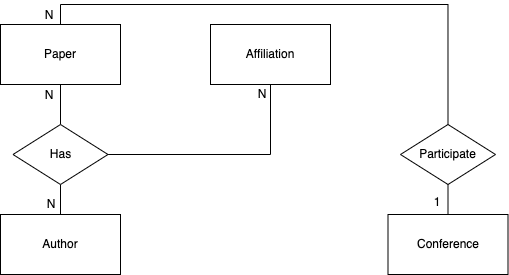
\includegraphics[width=0.8\linewidth]{./images/er1.png}
    \caption{Modello ER del problema}
    \label{fig:er1}
\end{figure}

\begin{figure}[h!]
    \centering
    \includegraphics[width=0.8\linewidth]{./images/er2.png}
    \caption{Modello ER del problema}
    \label{fig:er2}
\end{figure}


\begin{figure}[h!]
    \centering
    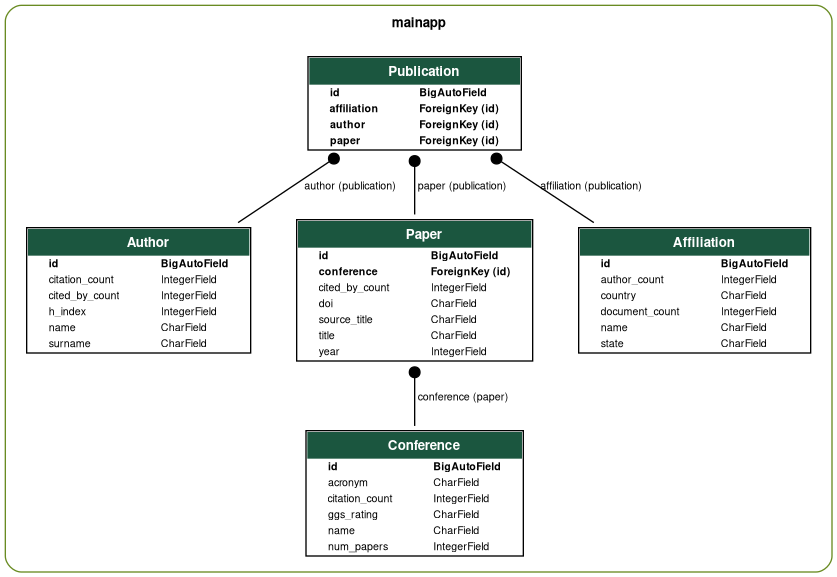
\includegraphics[width=0.8\linewidth]{./images/logico.png}
    \caption{Schema logico del problema}
    \label{fig:logico}
\end{figure}